% Options for packages loaded elsewhere
\PassOptionsToPackage{unicode}{hyperref}
\PassOptionsToPackage{hyphens}{url}
\PassOptionsToPackage{dvipsnames,svgnames,x11names}{xcolor}
%
\documentclass[
  letterpaper,
  DIV=11,
  numbers=noendperiod]{scrartcl}

\usepackage{amsmath,amssymb}
\usepackage{iftex}
\ifPDFTeX
  \usepackage[T1]{fontenc}
  \usepackage[utf8]{inputenc}
  \usepackage{textcomp} % provide euro and other symbols
\else % if luatex or xetex
  \usepackage{unicode-math}
  \defaultfontfeatures{Scale=MatchLowercase}
  \defaultfontfeatures[\rmfamily]{Ligatures=TeX,Scale=1}
\fi
\usepackage{lmodern}
\ifPDFTeX\else  
    % xetex/luatex font selection
\fi
% Use upquote if available, for straight quotes in verbatim environments
\IfFileExists{upquote.sty}{\usepackage{upquote}}{}
\IfFileExists{microtype.sty}{% use microtype if available
  \usepackage[]{microtype}
  \UseMicrotypeSet[protrusion]{basicmath} % disable protrusion for tt fonts
}{}
\makeatletter
\@ifundefined{KOMAClassName}{% if non-KOMA class
  \IfFileExists{parskip.sty}{%
    \usepackage{parskip}
  }{% else
    \setlength{\parindent}{0pt}
    \setlength{\parskip}{6pt plus 2pt minus 1pt}}
}{% if KOMA class
  \KOMAoptions{parskip=half}}
\makeatother
\usepackage{xcolor}
\setlength{\emergencystretch}{3em} % prevent overfull lines
\setcounter{secnumdepth}{-\maxdimen} % remove section numbering
% Make \paragraph and \subparagraph free-standing
\ifx\paragraph\undefined\else
  \let\oldparagraph\paragraph
  \renewcommand{\paragraph}[1]{\oldparagraph{#1}\mbox{}}
\fi
\ifx\subparagraph\undefined\else
  \let\oldsubparagraph\subparagraph
  \renewcommand{\subparagraph}[1]{\oldsubparagraph{#1}\mbox{}}
\fi

\usepackage{color}
\usepackage{fancyvrb}
\newcommand{\VerbBar}{|}
\newcommand{\VERB}{\Verb[commandchars=\\\{\}]}
\DefineVerbatimEnvironment{Highlighting}{Verbatim}{commandchars=\\\{\}}
% Add ',fontsize=\small' for more characters per line
\usepackage{framed}
\definecolor{shadecolor}{RGB}{241,243,245}
\newenvironment{Shaded}{\begin{snugshade}}{\end{snugshade}}
\newcommand{\AlertTok}[1]{\textcolor[rgb]{0.68,0.00,0.00}{#1}}
\newcommand{\AnnotationTok}[1]{\textcolor[rgb]{0.37,0.37,0.37}{#1}}
\newcommand{\AttributeTok}[1]{\textcolor[rgb]{0.40,0.45,0.13}{#1}}
\newcommand{\BaseNTok}[1]{\textcolor[rgb]{0.68,0.00,0.00}{#1}}
\newcommand{\BuiltInTok}[1]{\textcolor[rgb]{0.00,0.23,0.31}{#1}}
\newcommand{\CharTok}[1]{\textcolor[rgb]{0.13,0.47,0.30}{#1}}
\newcommand{\CommentTok}[1]{\textcolor[rgb]{0.37,0.37,0.37}{#1}}
\newcommand{\CommentVarTok}[1]{\textcolor[rgb]{0.37,0.37,0.37}{\textit{#1}}}
\newcommand{\ConstantTok}[1]{\textcolor[rgb]{0.56,0.35,0.01}{#1}}
\newcommand{\ControlFlowTok}[1]{\textcolor[rgb]{0.00,0.23,0.31}{#1}}
\newcommand{\DataTypeTok}[1]{\textcolor[rgb]{0.68,0.00,0.00}{#1}}
\newcommand{\DecValTok}[1]{\textcolor[rgb]{0.68,0.00,0.00}{#1}}
\newcommand{\DocumentationTok}[1]{\textcolor[rgb]{0.37,0.37,0.37}{\textit{#1}}}
\newcommand{\ErrorTok}[1]{\textcolor[rgb]{0.68,0.00,0.00}{#1}}
\newcommand{\ExtensionTok}[1]{\textcolor[rgb]{0.00,0.23,0.31}{#1}}
\newcommand{\FloatTok}[1]{\textcolor[rgb]{0.68,0.00,0.00}{#1}}
\newcommand{\FunctionTok}[1]{\textcolor[rgb]{0.28,0.35,0.67}{#1}}
\newcommand{\ImportTok}[1]{\textcolor[rgb]{0.00,0.46,0.62}{#1}}
\newcommand{\InformationTok}[1]{\textcolor[rgb]{0.37,0.37,0.37}{#1}}
\newcommand{\KeywordTok}[1]{\textcolor[rgb]{0.00,0.23,0.31}{#1}}
\newcommand{\NormalTok}[1]{\textcolor[rgb]{0.00,0.23,0.31}{#1}}
\newcommand{\OperatorTok}[1]{\textcolor[rgb]{0.37,0.37,0.37}{#1}}
\newcommand{\OtherTok}[1]{\textcolor[rgb]{0.00,0.23,0.31}{#1}}
\newcommand{\PreprocessorTok}[1]{\textcolor[rgb]{0.68,0.00,0.00}{#1}}
\newcommand{\RegionMarkerTok}[1]{\textcolor[rgb]{0.00,0.23,0.31}{#1}}
\newcommand{\SpecialCharTok}[1]{\textcolor[rgb]{0.37,0.37,0.37}{#1}}
\newcommand{\SpecialStringTok}[1]{\textcolor[rgb]{0.13,0.47,0.30}{#1}}
\newcommand{\StringTok}[1]{\textcolor[rgb]{0.13,0.47,0.30}{#1}}
\newcommand{\VariableTok}[1]{\textcolor[rgb]{0.07,0.07,0.07}{#1}}
\newcommand{\VerbatimStringTok}[1]{\textcolor[rgb]{0.13,0.47,0.30}{#1}}
\newcommand{\WarningTok}[1]{\textcolor[rgb]{0.37,0.37,0.37}{\textit{#1}}}

\providecommand{\tightlist}{%
  \setlength{\itemsep}{0pt}\setlength{\parskip}{0pt}}\usepackage{longtable,booktabs,array}
\usepackage{calc} % for calculating minipage widths
% Correct order of tables after \paragraph or \subparagraph
\usepackage{etoolbox}
\makeatletter
\patchcmd\longtable{\par}{\if@noskipsec\mbox{}\fi\par}{}{}
\makeatother
% Allow footnotes in longtable head/foot
\IfFileExists{footnotehyper.sty}{\usepackage{footnotehyper}}{\usepackage{footnote}}
\makesavenoteenv{longtable}
\usepackage{graphicx}
\makeatletter
\def\maxwidth{\ifdim\Gin@nat@width>\linewidth\linewidth\else\Gin@nat@width\fi}
\def\maxheight{\ifdim\Gin@nat@height>\textheight\textheight\else\Gin@nat@height\fi}
\makeatother
% Scale images if necessary, so that they will not overflow the page
% margins by default, and it is still possible to overwrite the defaults
% using explicit options in \includegraphics[width, height, ...]{}
\setkeys{Gin}{width=\maxwidth,height=\maxheight,keepaspectratio}
% Set default figure placement to htbp
\makeatletter
\def\fps@figure{htbp}
\makeatother
\newlength{\cslhangindent}
\setlength{\cslhangindent}{1.5em}
\newlength{\csllabelwidth}
\setlength{\csllabelwidth}{3em}
\newlength{\cslentryspacingunit} % times entry-spacing
\setlength{\cslentryspacingunit}{\parskip}
\newenvironment{CSLReferences}[2] % #1 hanging-ident, #2 entry spacing
 {% don't indent paragraphs
  \setlength{\parindent}{0pt}
  % turn on hanging indent if param 1 is 1
  \ifodd #1
  \let\oldpar\par
  \def\par{\hangindent=\cslhangindent\oldpar}
  \fi
  % set entry spacing
  \setlength{\parskip}{#2\cslentryspacingunit}
 }%
 {}
\usepackage{calc}
\newcommand{\CSLBlock}[1]{#1\hfill\break}
\newcommand{\CSLLeftMargin}[1]{\parbox[t]{\csllabelwidth}{#1}}
\newcommand{\CSLRightInline}[1]{\parbox[t]{\linewidth - \csllabelwidth}{#1}\break}
\newcommand{\CSLIndent}[1]{\hspace{\cslhangindent}#1}

\KOMAoption{captions}{tableheading}
\makeatletter
\makeatother
\makeatletter
\makeatother
\makeatletter
\@ifpackageloaded{caption}{}{\usepackage{caption}}
\AtBeginDocument{%
\ifdefined\contentsname
  \renewcommand*\contentsname{Table of contents}
\else
  \newcommand\contentsname{Table of contents}
\fi
\ifdefined\listfigurename
  \renewcommand*\listfigurename{List of Figures}
\else
  \newcommand\listfigurename{List of Figures}
\fi
\ifdefined\listtablename
  \renewcommand*\listtablename{List of Tables}
\else
  \newcommand\listtablename{List of Tables}
\fi
\ifdefined\figurename
  \renewcommand*\figurename{Figure}
\else
  \newcommand\figurename{Figure}
\fi
\ifdefined\tablename
  \renewcommand*\tablename{Table}
\else
  \newcommand\tablename{Table}
\fi
}
\@ifpackageloaded{float}{}{\usepackage{float}}
\floatstyle{ruled}
\@ifundefined{c@chapter}{\newfloat{codelisting}{h}{lop}}{\newfloat{codelisting}{h}{lop}[chapter]}
\floatname{codelisting}{Listing}
\newcommand*\listoflistings{\listof{codelisting}{List of Listings}}
\makeatother
\makeatletter
\@ifpackageloaded{caption}{}{\usepackage{caption}}
\@ifpackageloaded{subcaption}{}{\usepackage{subcaption}}
\makeatother
\makeatletter
\@ifpackageloaded{tcolorbox}{}{\usepackage[skins,breakable]{tcolorbox}}
\makeatother
\makeatletter
\@ifundefined{shadecolor}{\definecolor{shadecolor}{rgb}{.97, .97, .97}}
\makeatother
\makeatletter
\makeatother
\makeatletter
\makeatother
\ifLuaTeX
  \usepackage{selnolig}  % disable illegal ligatures
\fi
\IfFileExists{bookmark.sty}{\usepackage{bookmark}}{\usepackage{hyperref}}
\IfFileExists{xurl.sty}{\usepackage{xurl}}{} % add URL line breaks if available
\urlstyle{same} % disable monospaced font for URLs
\hypersetup{
  pdftitle={A simple NPZD model for Llanquihue Lake},
  pdfauthor={Carolina Rösner \& Rodrigo Jaramillo Teufert},
  colorlinks=true,
  linkcolor={blue},
  filecolor={Maroon},
  citecolor={Blue},
  urlcolor={Blue},
  pdfcreator={LaTeX via pandoc}}

\title{A simple NPZD model for Llanquihue Lake}
\author{Carolina Rösner \& Rodrigo Jaramillo Teufert}
\date{}

\begin{document}
\maketitle
\ifdefined\Shaded\renewenvironment{Shaded}{\begin{tcolorbox}[breakable, sharp corners, boxrule=0pt, frame hidden, enhanced, interior hidden, borderline west={3pt}{0pt}{shadecolor}]}{\end{tcolorbox}}\fi

\hypertarget{abstract}{%
\section{Abstract}\label{abstract}}

In the present study, a mathematical model (NPZD) based on the four
compartments Nutrient (N), Phytoplankton (P), Zooplankton (Z) and
Detritus (D), is proposed for understanding the ecology of shallow
coastal lagoons. Model is simulated for the two cases of detritus link
with the system: i) through remineralization and ii) through
remineralization and palatability of detritus to zooplankton.

\hypertarget{introduction}{%
\subsection{Introduction}\label{introduction}}

A biogeochemical model is a simplified and mathematical representation
of the biological, geological, and chemical processes that occur in
ecosystems. These models are used to understand and simulate the flows
of energy, nutrients, and chemical elements through natural systems such
as oceans, forests, soils, and bodies of water. Biogeochemical models
integrate information about biogeochemical cycles, which include
processes like photosynthesis, decomposition, respiration, nitrogen
fixation, nutrient leaching, and atmospheric deposition.

These models take into account the interactions between different
components of the system, such as plants, animals, microorganisms,
soils, and the atmosphere. Biogeochemical models are powerful tools for
predicting the effects of environmental change, such as climate change,
pollution, and deforestation, on biogeochemical cycles and ecosystem
health. They are also used to assess the effectiveness of management and
conservation strategies and to inform decision-making in natural
resource management.

Biological models have been widely used to understand the dynamics and
interactions in pelagic ecosystems. Among them, compartmental models
have been especially relevant by grouping entire populations into
individual compartments that interact with each other. The complexity of
these models varies depending on the included state variables and the
rules governing their interaction. One known model in this context is
the model proposed by Fasham et al.~(1990), which includes seven
compartments: phytoplankton, zooplankton, bacteria, nitrate, ammonium,
dissolved organic nitrogen, and detritus. However, one of the simplest
and most widely used biological models is the NPZ model developed by
Franks et al.~(1986), which considers only three compartments:
phytoplankton, zooplankton, and dissolved nutrients.

The NPZ model captures the fundamental processes governing the growth
and interactions between these key compartments. It considers variables
such as nutrient availability, grazing pressure, and phytoplankton
growth rates, providing a simplified yet valuable representation of
pelagic ecosystem dynamics. This model has been adapted and applied in
various marine environments, providing crucial insights into the
functioning of planktonic communities and their responses to
environmental changes.

In conclusion, biological models like the NPZ model play a crucial role
in our understanding of the complex dynamics and interactions in pelagic
ecosystems. While more complex models encompass multiple compartments
and variables, the NPZ model provides an effective and simplified
representation of essential components in these ecosystems. These models
are valuable tools for advancing our knowledge and contributing to the
conservation and management of marine habitats.

\textbf{2. Model Formulation}

A mathematical model (NPZD) based on four compartments (Nutrient (N),
Phytoplankton (P), Zooplankton (Z), and Detritus (D)) is proposed to
understand the ecology of shallow coastal zones and lagoons. The
interactions between the compartments are described in Figure 1.

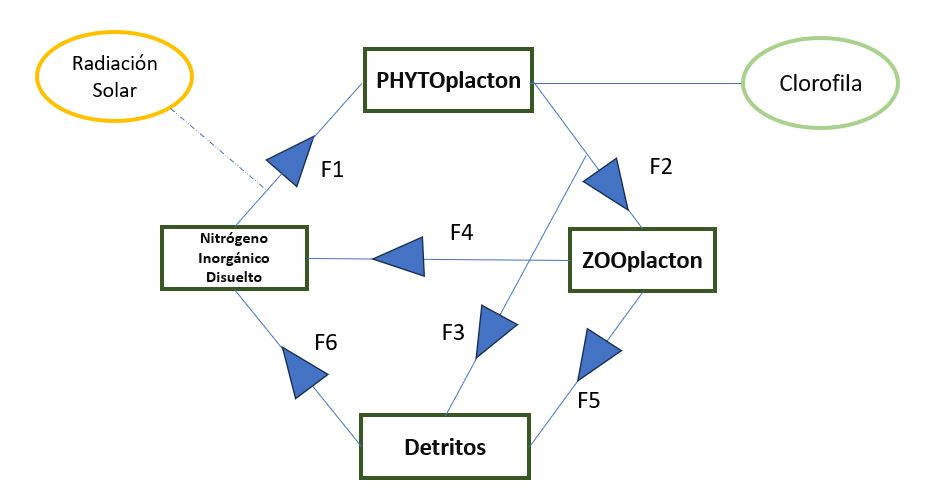
\includegraphics{NPZD.JPG}

The arrows indicate the flow of matter between different compartments.
The equations of the model are as follows:

\(dN/dt= - (a(t)NP)/(Kn+N) + rP + øD + [m/H(t)]N1 (t) + (Q/V)N2(t)\)

\(dP/dt=\)

\(dZ/dt=\)

\(dD/dt=\)

All parameters, along with their units and ranges, are provided in Table
1. The units for N, P, Z, and D are µg/l, and the unit of time is in
days. The parameterization used to select the terms in equations (1) -
(4) is explained in the sections\ldots..

\textbf{3. RESULTs}

\textbf{4. CONCLUSIONs}

\textbf{5. BIBLIOGRAFIA}

(Roy et al. 2012a)

{[}Chakraborty and Chattopadhyay (2008); Carlotti, Giske, and Werner
(2000){]}(A. M. Edwards and Brindley 1996; Chakraborty and Chattopadhyay
2008; Rudnicki and Wieczorek 2008; Record, Pershing, and Maps 2014; Roy
et al. 2012b; Priyadarshi et al. 2022; Olivieri and Chavez 2000;
Montagnes and Fenton 2012; Mitra 2009; Mitra, Flynn, and Fasham 2007;
Merico et al. 2014; Mandal, Ray, and Ghosh 2012; Lewis 2005; Leles,
VaLEntin, and FiGuEirEdo 2016; Lai et al. 2010; Kloosterman, Campbell,
and Poulin 2016; Jiang, Schofield, and Falkowski 2005; Giricheva 2019;
Gentleman and Neuheimer 2008; Franks 2002; A. M. Edwards 2001; C. A.
Edwards, Powell, and Batchelder 2000; Daewel et al. 2014; Carlotti,
Giske, and Werner 2000; Qiu and Zhu 2016; Rani and Jayaraman 2010;
Sanson and Provenzale 2009; Serra-Pompei et al. 2020; Steele and
Henderson 1992; Turner et al. 2014)

\begin{Shaded}
\begin{Highlighting}[]
\DecValTok{1} \SpecialCharTok{+} \DecValTok{1}
\end{Highlighting}
\end{Shaded}

\begin{verbatim}
[1] 2
\end{verbatim}

\hypertarget{refs}{}
\begin{CSLReferences}{1}{0}
\leavevmode\vadjust pre{\hypertarget{ref-carlotti2000}{}}%
Carlotti, Francois, J. Giske, and Felix Werner. 2000. {``Modeling
Zooplankton Dynamics.''} In, 571667. Elsevier.

\leavevmode\vadjust pre{\hypertarget{ref-chakraborty2008}{}}%
Chakraborty, Subhendu, and Joydev Chattopadhyay. 2008.
{``Nutrient-Phytoplankton-Zooplankton Dynamics in the Presence of
Additional Food Source{\textemdash}a Mathematical Study.''}
\emph{Journal of Biological Systems} 16 (04): 547564.

\leavevmode\vadjust pre{\hypertarget{ref-daewel2014}{}}%
Daewel, Ute, Solfrid Sætre Hjøllo, Martin Huret, Rubao Ji, Marie Maar,
Susa Niiranen, Morgane Travers-Trolet, Myron A. Peck, and Karen E. van
de Wolfshaar. 2014. {``Predation Control of Zooplankton Dynamics: A
Review of Observations and Models.''} \emph{ICES Journal of Marine
Science} 71 (2): 254271.

\leavevmode\vadjust pre{\hypertarget{ref-edwards2001}{}}%
Edwards, Andrew M. 2001. {``Adding Detritus to a
Nutrient{\textendash}phytoplankton{\textendash}zooplankton Model: A
Dynamical-Systems Approach.''} \emph{Journal of Plankton Research} 23
(4): 389413.

\leavevmode\vadjust pre{\hypertarget{ref-edwards1996}{}}%
Edwards, Andrew M., and John Brindley. 1996. {``Oscillatory Behaviour in
a Three-Component Plankton Population Model.''} \emph{Dynamics and
Stability of Systems} 11 (4): 347370.

\leavevmode\vadjust pre{\hypertarget{ref-edwards2000}{}}%
Edwards, Christopher A., Thomas A. Powell, and Harold P. Batchelder.
2000. {``The Stability of an NPZ Model Subject to Realistic Levels of
Vertical Mixing.''} \emph{Journal of Marine Research} 58 (1): 3760.

\leavevmode\vadjust pre{\hypertarget{ref-franks2002}{}}%
Franks, Peter JS. 2002. {``NPZ Models of Plankton Dynamics: Their
Construction, Coupling to Physics, and Application.''} \emph{Journal of
Oceanography} 58: 379387.

\leavevmode\vadjust pre{\hypertarget{ref-gentleman2008}{}}%
Gentleman, W. C., and A. B. Neuheimer. 2008. {``Functional Responses and
Ecosystem Dynamics: How Clearance Rates Explain the Influence of
Satiation, Food-Limitation and Acclimation.''} \emph{Journal of Plankton
Research} 30 (11): 12151231.

\leavevmode\vadjust pre{\hypertarget{ref-giricheva2019}{}}%
Giricheva, Evgeniya. 2019. {``Spatiotemporal Dynamics of an NPZ Model
with Prey-Taxis and Intratrophic Predation.''} \emph{Nonlinear Dynamics}
95 (2): 875892.

\leavevmode\vadjust pre{\hypertarget{ref-jiang2005}{}}%
Jiang, Lin, Oscar ME Schofield, and Paul G. Falkowski. 2005. {``Adaptive
Evolution of Phytoplankton Cell Size.''} \emph{The American Naturalist}
166 (4): 496505.

\leavevmode\vadjust pre{\hypertarget{ref-kloosterman2016}{}}%
Kloosterman, Matt, Sue Ann Campbell, and Francis J. Poulin. 2016. {``An
NPZ Model with State-Dependent Delay Due to Size-Structure in Juvenile
Zooplankton.''} \emph{SIAM Journal on Applied Mathematics} 76 (2):
551577.

\leavevmode\vadjust pre{\hypertarget{ref-lai2010}{}}%
Lai, Zhigang, Changsheng Chen, Robert C. Beardsley, Brian Rothschild,
and Rucheng Tian. 2010. {``Impact of High-Frequency Nonlinear Internal
Waves on Plankton Dynamics in Massachusetts Bay.''} \emph{Journal of
Marine Research} 68 (2): 259281.

\leavevmode\vadjust pre{\hypertarget{ref-leles2016}{}}%
Leles, Suzana G., JEan L. VaLEntin, and GiSELa M. FiGuEirEdo. 2016.
{``Evaluation of the Complexity and Performance of Marine Planktonic
Trophic Models.''} \emph{Anais Da Academia Brasileira de Ciências} 88:
19711991.

\leavevmode\vadjust pre{\hypertarget{ref-lewis2005}{}}%
Lewis, D. M. 2005. {``A Simple Model of Plankton Population Dynamics
Coupled with a LES of the Surface Mixed Layer.''} \emph{Journal of
Theoretical Biology} 234 (4): 565591.

\leavevmode\vadjust pre{\hypertarget{ref-mandal2012}{}}%
Mandal, Sudipto, Santanu Ray, and Phani Bhusan Ghosh. 2012. {``Modeling
Nutrient (Dissolved Inorganic Nitrogen) and Plankton Dynamics at Sagar
Island of Hooghly{\textendash}matla Estuarine System, West Bengal,
India.''} \emph{Natural Resource Modeling} 25 (4): 629652.

\leavevmode\vadjust pre{\hypertarget{ref-merico2014}{}}%
Merico, Agostino, Gunnar Brandt, S. Lan Smith, and Marcel Oliver. 2014.
{``Sustaining Diversity in Trait-Based Models of Phytoplankton
Communities.''} \emph{Frontiers in Ecology and Evolution} 2: 59.

\leavevmode\vadjust pre{\hypertarget{ref-mitra2009}{}}%
Mitra, Aditee. 2009. {``Are Closure Terms Appropriate or Necessary
Descriptors of Zooplankton Loss in
Nutrient{\textendash}phytoplankton{\textendash}zooplankton Type
Models?''} \emph{Ecological Modelling} 220 (5): 611620.

\leavevmode\vadjust pre{\hypertarget{ref-mitra2007}{}}%
Mitra, Aditee, Kevin J. Flynn, and Michael JR Fasham. 2007.
{``Accounting for Grazing Dynamics in Nitrogen-Phytoplankton-Zooplankton
(NPZ) Models.''} \emph{Limnology and Oceanography} 52 (2): 649661.

\leavevmode\vadjust pre{\hypertarget{ref-montagnes2012}{}}%
Montagnes, David JS, and Andy Fenton. 2012. {``Prey-Abundance Affects
Zooplankton Assimilation Efficiency and the Outcome of Biogeochemical
Models.''} \emph{Ecological Modelling} 243: 17.

\leavevmode\vadjust pre{\hypertarget{ref-olivieri2000}{}}%
Olivieri, Rafael A., and Francisco P. Chavez. 2000. {``A Model of
Plankton Dynamics for the Coastal Upwelling System of Monterey Bay,
California.''} \emph{Deep Sea Research Part II: Topical Studies in
Oceanography} 47 (5-6): 10771106.

\leavevmode\vadjust pre{\hypertarget{ref-priyadarshi2022}{}}%
Priyadarshi, Anupam, Ram Chandra, Michio J. Kishi, S. Lan Smith, and
Hidekatsu Yamazaki. 2022. {``Understanding Plankton Ecosystem Dynamics
Under Realistic Micro-Scale Variability Requires Modeling at Least Three
Trophic Levels.''} \emph{Ecological Modelling} 467: 109936.

\leavevmode\vadjust pre{\hypertarget{ref-qiu2016}{}}%
Qiu, Zhipeng, and Huaiping Zhu. 2016. {``Complex Dynamics of a
Nutrient-Plankton System with Nonlinear Phytoplankton Mortality and
Allelopathy.''} \emph{Discrete and Continuous Dynamical
Systems{\textemdash}Series B} 21 (8): 27032728.

\leavevmode\vadjust pre{\hypertarget{ref-rani2010}{}}%
Rani, Raj, and Girija Jayaraman. 2010. {``A Minimal Model for Plankton
Dynamics in Shallow Coastal Lagoons-Chilika Lagoon, a Case Study.''}
\emph{International Journal of Emerging Multidisciplinary Fluid
Sciences} 2.

\leavevmode\vadjust pre{\hypertarget{ref-record2014}{}}%
Record, Nicholas R., Andrew J. Pershing, and Frédéric Maps. 2014. {``The
Paradox of the {``}Paradox of the Plankton{''}.''} \emph{ICES Journal of
Marine Science} 71 (2): 236240.

\leavevmode\vadjust pre{\hypertarget{ref-roy2012}{}}%
Roy, Shovonlal, David S. Broomhead, Trevor Platt, Shubha Sathyendranath,
and Stefano Ciavatta. 2012a. {``Sequential Variations of Phytoplankton
Growth and Mortality in an NPZ Model: A Remote-Sensing-Based
Assessment.''} \emph{Journal of Marine Systems} 92 (1): 1629.

\leavevmode\vadjust pre{\hypertarget{ref-roy2012a}{}}%
---------. 2012b. {``Sequential Variations of Phytoplankton Growth and
Mortality in an NPZ Model: A Remote-Sensing-Based Assessment.''}
\emph{Journal of Marine Systems} 92 (1): 1629.

\leavevmode\vadjust pre{\hypertarget{ref-rudnicki2008}{}}%
Rudnicki, Ryszard, and Radosáaw Wieczorek. 2008. {``Mathematical Models
of Phytoplankton Dynamics.''} \emph{Dynamic Biochemistry, Process
Biotechnology and Molecular Biology} 2 (1): 5563.

\leavevmode\vadjust pre{\hypertarget{ref-sanson2009}{}}%
Sanson, L. Zavala, and A. Provenzale. 2009. {``The Effects of Abrupt
Topography on Plankton Dynamics.''} \emph{Theoretical Population
Biology} 76 (4): 258267.

\leavevmode\vadjust pre{\hypertarget{ref-serra-pompei2020}{}}%
Serra-Pompei, Camila, Floor Soudijn, André W. Visser, Thomas Kiørboe,
and Ken H. Andersen. 2020. {``A General Size-and Trait-Based Model of
Plankton Communities.''} \emph{Progress in Oceanography} 189: 102473.

\leavevmode\vadjust pre{\hypertarget{ref-steele1992}{}}%
Steele, John H., and Eric W. Henderson. 1992. {``The Role of Predation
in Plankton Models.''} \emph{Journal of Plankton Research} 14 (1):
157172.

\leavevmode\vadjust pre{\hypertarget{ref-turner2014}{}}%
Turner, Evan L., Denise A. Bruesewitz, Rae F. Mooney, Paul A. Montagna,
James W. McClelland, Alexey Sadovski, and Edward J. Buskey. 2014.
{``Comparing Performance of Five Nutrient Phytoplankton Zooplankton
(NPZ) Models in Coastal Lagoons.''} \emph{Ecological Modelling} 277:
1326.

\end{CSLReferences}



\end{document}
